

\documentclass[11pt]{article}
\usepackage{graphicx}
\usepackage{times}
\usepackage{amssymb}
\usepackage{float}
\usepackage{amsmath,amssymb,amsfonts,bm}

\newcount\refno\refno=1
\def\ref{\the\refno \global\advance\refno by 1}
\def\ux{\underline{x}}
\def\uw{\underline{w}}
\def\ut{\underline{\theta}}
\def\umu{\underline{\mu}}
\def\be{p_e^*}
\newcount\eqnumber\eqnumber=1
\def\eq{\the \eqnumber \global\advance\eqnumber by 1}
\def\eqs{\eq}
\def\eqn{\eqno(\eq)}

 \pagestyle{empty}
\def\baselinestretch{1.1}
\topmargin1in \headsep0.3in
\topmargin0in \oddsidemargin0in \textwidth6.5in \textheight8.5in
\begin{document}
\setlength{\parskip}{1.2ex plus0.3ex minus 0.3ex}


\thispagestyle{empty} \pagestyle{myheadings} \markright{Homework
2: CS 274A, Probabilistic Learning: Winter 2019}



\title{CS 274A Homework 2}
\author{Caleb Nelson}
\date{Due Date:  11am Wednesday January 23rd}

\maketitle


\section*{Instructions and Guidelines for Homeworks}
 \begin{itemize}

\item
Please answer all of the questions and submit a scanned copy of your written solutions to Gradescope 
(either hand-written or typed are fine as long as the writing is legible). 
%Code (if requested) should be submitted to the EEE dropbox. No
%need to submit any code unless we request it.

\item
All problems are worth 10 points unless otherwise stated.  All homeworks will get equal weight in computation of the final grade for the class.
 \item
The homeworks are intended to help you work through the concepts
we discuss in class in  more detail. It is important that you try
to solve the problems yourself. The homework problems are important to help you better
learn and reinforce the material from class. If you don't
do the homeworks you will likely have difficulty in the exams
later in the quarter.

\item If you can't solve a
problem, you can discuss it {\it verbally} with another student. However, please note that before you submit your homework solutions you
are not allowed to view (or show to any other student) any {\it written material} directly related to the homeworks, including other students' solutions or drafts of solutions, solutions from previous versions of this class, and so forth. The work you hand in should be your own original work.

\item You are allowed to use reference materials in your solutions, such as class notes, textbooks,  other reference material (e.g., from the Web), or solutions to other problems in the homework. It is strongly recommended that you first try to solve the problem yourself, without resorting to looking up solutions elsewhere. If you base your solution on material that we did not discuss in class, or is not in the class notes, then you need to clearly provide a reference, e.g., ``based on material in Section 2.2 in ....."


\item
In problems that ask for a proof you should submit a complete mathematical
proof (i.e., each line must follow logically from the preceding one, without
``hand-waving"). Be as clear as possible in explaining
 your notation and in stating your reasoning as you go from line to line.  


\item
If you wish to use LaTeX to write up
your solutions you may find it useful to use the .tex file for  this homework
that is posted on the Web page. 






\end{itemize}



\subsection*{Problem \ref: (Finite Mixture Models)}
Finite mixture models show up in a wide variety of contexts in machine learning and statistics (we will discuss them in more detail in lectures later in the quarter). In this problem consider a real-valued random variable $X$ taking values $x$ (in general we can define mixtures on vectors, but here we will just consider the 1-dimensional scalar case). The basic idea is to define a density (or distribution) $p(x)$ that is a weighted mixture of $K$ component densities $p_k(x)$ where the weights are non-negative and sum to 1, i.e.,
\[
p(x)  \ = \ \sum_{k=1}^K \alpha_k \ p_k(x; \theta_k)
\]
where 
\begin{itemize}
\item the weights obey the following conditions: $\sum_{k=1}^K \alpha_k = 1, \ \  0 \le \alpha_k \le 1$
\item each $p_k(x; \theta_k)$ is itself a probability density function with its own parameters $\theta_k$. For example, if a component is Gaussian then $\theta_k = \{\mu_k, \sigma^2_k\}$.
 \end{itemize}
 The full set of parameters for a mixture model consists of both (a) the $K$ weights, and (b) the $K$ sets of component parameters $\theta_k$ for each of the $K$ mixture components.
 (Note that the ``finite" in finite mixture models comes from the fact that $K$ is finite. There are also infinite mixture models where $K$ is unbounded, but we will not consider those here).
  
 \begin{enumerate}
\item Given the properties above prove that a finite mixture $p(x)$ is itself a density function, i.e., it obeys all the necessary properties needed to be a density function. 

Since $p(x)$ is composed of continuous functions, it is trivially continuous everywhere. 
Since every $p_k(x)$ is a pdf, $\int_0^1 p_k(x) = 1$ for every $k$. 
Thus, $\int_0^1 p(x) = \sum_{k=1}^K \alpha_k \int_0^1 p_k(x) = \sum_{k=1}^K \alpha_k * 1 = 1$.
Therefore $p(x)$ is a valid pdf.

\item Derive general expressions for the (a) mean $\mu$ of $p(x)$, and
(b) the variance $\sigma^2$ of $p(x)$, as a function of the
component weights, means and variances $\alpha_k, \mu_k, \sigma_k^2, 1 \le k \le K$. For
each of $\mu$  and $\sigma^2$ provide an intuitive interpretation in words of your solutions.

$\mu = \sum_{k=1}^K \alpha_k \mu_k$. This makes intuitive sense, as the mean of the mixture model 
would naturally be the average of the means of the distributions that make up the model, weighted 
by how much influence each distribution has on the model.
\begin{equation}
\sigma^2 = E[x^2] - E[x]^2 = 
\sum_{k=1}^K \alpha_k (\sigma_k^2 + \mu_k^2) - (\sum_{k=1}^K \alpha_k \mu_k)^2 = 
\sum_{k=1}^K \alpha_k \sigma_k^2 + \sum_{k=1}^K \alpha_k \mu_k^2 - (\sum_{k=1}^K \alpha_k \mu_k)^2
\end{equation}
The intuition behind this result is that since $\sum_{k=1}^K \alpha_k \mu_k^2 - (\sum_{k=1}^K \alpha_k \mu_k)^2 \geq 0$ and equal to zero when all $\mu_k$'s overlap, this new variance represents the combined variances with an added parameter that represents the extra variance caused by the distance between means.

\item 
\begin{itemize}
\item In the case that each of the components  $p_k(x)$ are unimodal (i.e., have a unique mode), what is the minimum and maximum number of modes in general that the mixture density can have (you can assume here that each $\alpha_k > 0)$. You can just state your answer.

The number of modes is between 1 and K.

\item For a mixture density with Gaussian components and $K=3$, provide  examples of values for the mixture parameter values that clearly illustrate both cases (i.e., minimum and maximum number of modes) and provide two figures (one for each case) that clearly plot the mixture density as well as its components (so each plot should have 4 densities overlaid: the mixture density and its 3 components).

For one mode, $p_k(x) = \mathcal{N}(0, k)$ for all k. For $K=3$ modes, $p_1(x) = \mathcal{N}(0, 1), p_2(x) = \mathcal{N}(-4, 1), p_3 = \mathcal{N}(4, 1)$

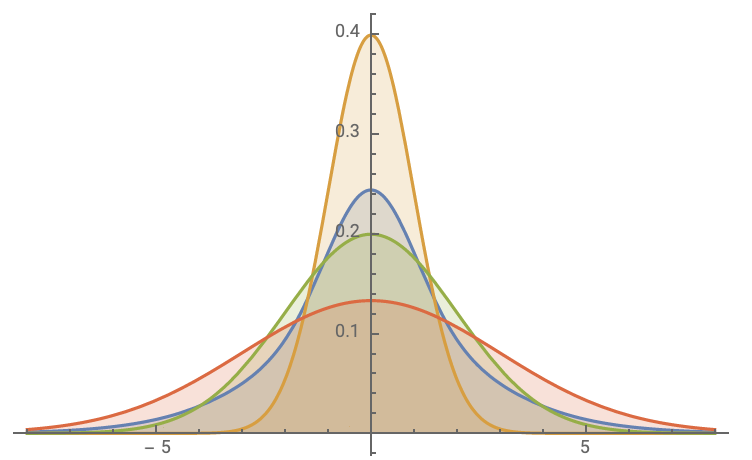
\includegraphics[scale=0.5]{graph1.png} 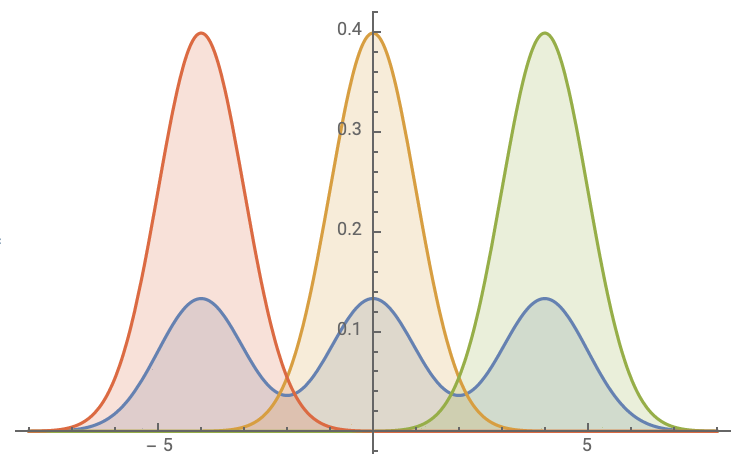
\includegraphics[scale=0.5]{graph2.png}

\end{itemize}

\end{enumerate}
 
 

\subsection*{Problem \ref: (Hidden Markov Models)}
Hidden Markov models are widely used in speech recognition, language modeling, genomics, time-series modeling, and many other applications. To define a hidden Markov model (HMM) we have two types of random variables:
\begin{enumerate}
\item $X_1,\ldots,X_T$ the hidden states, and
\item $Y_1,\ldots,Y_T$ the observations
\end{enumerate}
The index $t=1,\ldots,T$ could be discrete-time (e.g., every day) or just be an index on the order or position in a sequence---we will just refer to $t$ as time below. We will assume below that each $X_t$ variable is discrete taking $K$ values (sometimes these variables are referred to as ``states").  In general each $Y_t$ variable can be a vector of length $d$ with components that can be discrete or continuous or a mixture of each.

There are two conditional independence assumptions in an HMM. The first is a Markov assumption on the hidden $X$ variables:
\[ P(X_t | X_{t-1},\ldots,X_1) = P(X_t | X_{t-1}), \ \ \ \ t=2,\ldots,T \]
and where $P(X_1)$ has its own distribution (referred to as the initial state distribution).

The second assumption is that each $Y_t$ is conditionally independent of all other variables given $X_t$, i.e.,
\[
P(Y_t | X_1,\ldots,X_T, \mbox{other Y's}) =
P(Y_t | X_t),  \ \ \ \ t = 1,\ldots, T
\]
Thus, each $Y_t$ only depends on the state $X_t$ at time $t$.
 
 The parameters of an HMM consist of:
 (i) an initial state distribution $P(X_1)$, 
 (ii) a transition matrix $P(X_{t+1} = j | X_{t} = i), 1 \le i, j, \le K$, and
 (iii) parameters for the conditional densities $P(Y_t | X_t = k)$ of the observations given each possible state value, $1 \le k \le K$.
 The model is called {\it homogeneous} when $P(X_{t+1} = j | X_{t} = i)$ and 
 $P(Y_t | X_t = k)$  do not change as a function of $t$. In all the problems below you can assume the HMM is homogeneous.

(Sidenote: In answering this question you can (if you wish to) consult Note Set 5 on HMMs (on the class Website)---it uses  different notation to the notation here. However, note that this is just an option---its not necessary to read Note Set 5 to answer this question).

\begin{enumerate}

\item  
Draw a picture of the graphical model and write down an equation for the joint distribution of $X$'s and $Y$'s based on
the graphical model structure.

\item Say each $P(Y_t | X_t = k)$ is a Gaussian density (for real-valued $y_t$'s) for 2 different cases: (a) diagonal covariance matrices, (b)   full covariance matrices, where the $y_t$'s  are $d$-dimensional real-valued vectors. For each case (a) and (b) define precisely how many parameters we need in order to specify the HMM.
%\end{enumerate}
%\subsection*{Problem \ref: (Hidden Markov Models)}
%This is a continuation of the last problem.
%\begin{enumerate}
\item Consider a small toy example with $T=5$, i.e., sequences of length 5. Show systematically how one can compute $P(x_5 = k| y_1,\ldots,y_5), \ 1 \le k \le K$. Hint 1: work with joint probabilities and then normalize  to get the conditional probability of interest at the end. Hint 2: start with $P(X_2, y_1, y_2)$, use this to find $P(X_3, y_1,y_2, y_3)$, and so on. You can use $\sum_{x_t}$ or $\int_{y_t} dy_t$ to indicate summing or integrating over variables such as $x_t$ or $y_t$ respectively.

%\item Now say we know that $X_1=x^*_1$ and $X_3=x^*_3$ for some values of $X_1$ and $X_3$. Explain clearly how this would modify your solution to the last problem.

%\item Describe briefly how you could compute $P(X_3| y_1,\ldots,y_5)$ given $X_4 = x^*_4$ and $X_1 = x^*_1$. (No need to show all the details, just clearly describe what the key steps are in doing this calculation).
 
 \end{enumerate}
 
 
 \subsection*{Problem \ref: (Likelihood Functions)}
Consider the following data set $D=\{4, 8, 6, 8, 9, 12, 10, 6, 9,
7\}$. Use MATLAB (or python, or R, or something similar)
to generate graphs of the log-likelihood function for each of the following cases:
\begin{enumerate}
\item a Gaussian density with $\mu$ as the unknown parameter in the log-likelihood function
and with a fixed standard deviation of $\sigma = 3$.

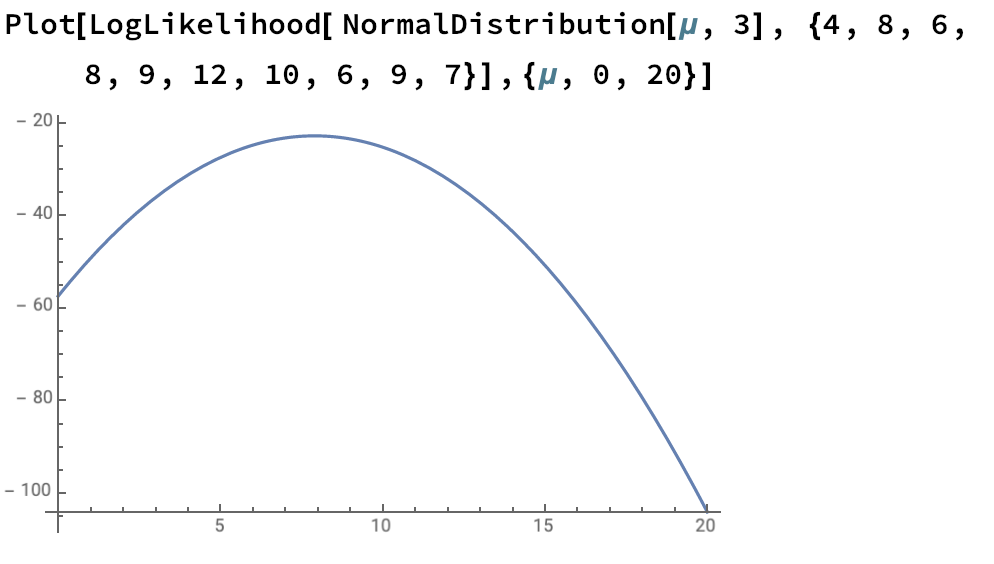
\includegraphics[scale=0.5]{three1.png} \\
This graph seems pretty ordinary, peaking at 7.9, the mean of the data set.

\item a uniform density with $a=3$ and $b$ as the unknown parameter in the log-likelihood function

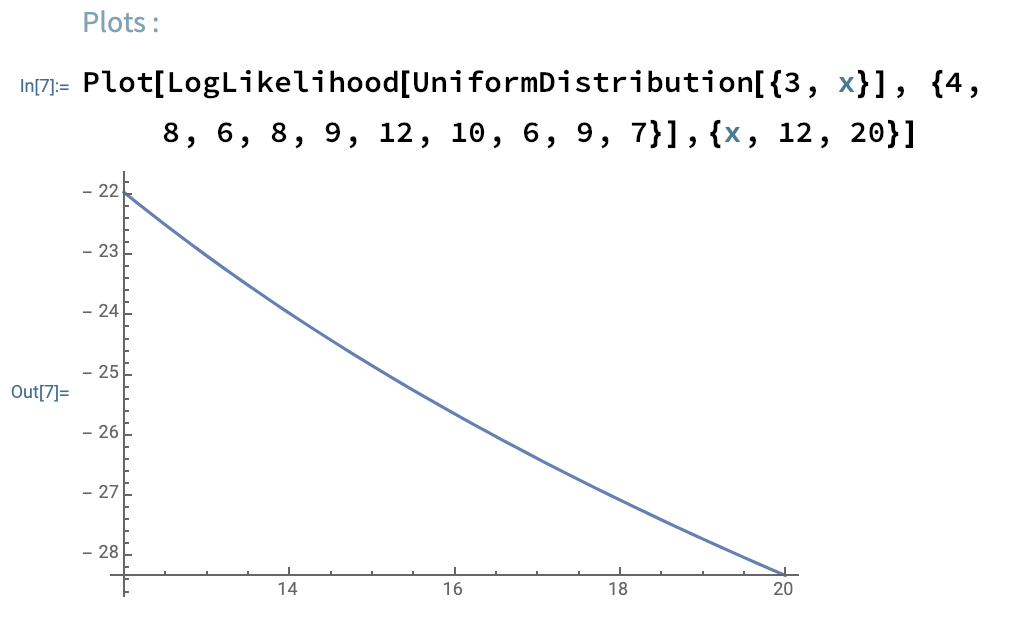
\includegraphics[scale=0.5]{three2.png} \\
This graph peaks at 12, which is the lowest value the parameter could possibly have due to the data set 
having an upper bound of 12.

\item an exponential density with the exponential parameter as the unknown parameter in the log-likelihood function.

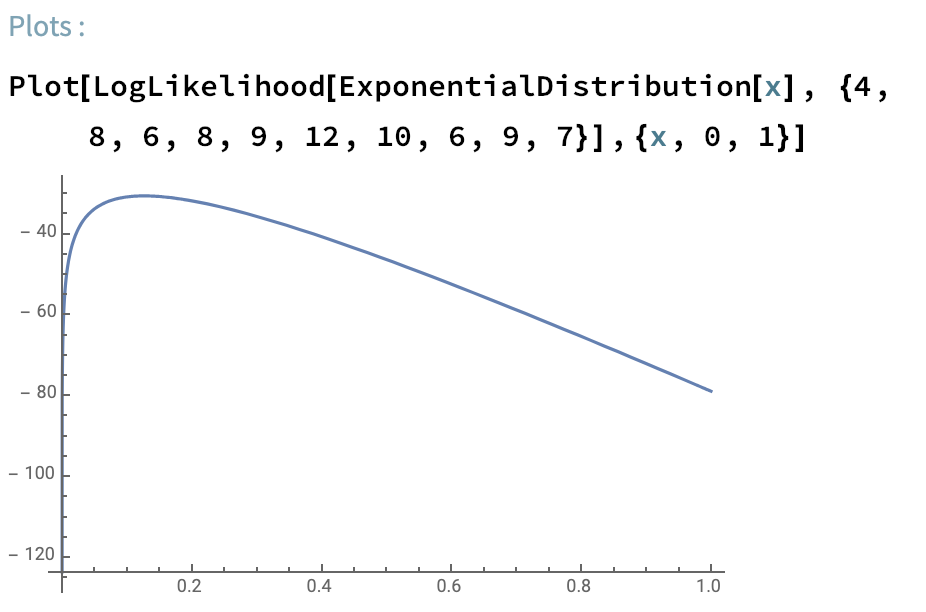
\includegraphics[scale=0.5]{three3.png} \\
This graph increases sharply and peaks quickly, but then begins a gradual decline that will continue for the rest of its life. The peak appears to be at around 0.1.
\end{enumerate}
In each case you can the plot a range of values around the mode of the log-likelihood function,
e.g., if $\theta$ is the mode you could plot in the range $[0.2\theta, 2\theta]$ (or something similar). 
Comment on the shape of each of the 3 plots.  
 
\vskip 1cm
 \noindent{\bf Note:} In the next few problems
below, unless otherwise stated, assume that
  a data set $D = \{x_1,\ldots,x_n\}$ exists.  You can also assume
that   the $x_i$'s are conditionally independent of each other
given the parameters of the model.
 
 



\subsection*{Problem \ref: (Maximum Likelihood for the Geometric Model)}
Derive the maximum-likelihood estimator for the geometric
distribution with parameter $p$, where the geometric distribution is defined as 
\[
P(X = k) \ = \ (1-p)^k p \ \ \ \ , k = 0,1, 2, 3, \ldots, \ \ \ 0 < p < 1
\] 

$L(\theta) = \prod_i^n P(x_i | \theta) = \theta^n(1-\theta)^{\sum_i^n x_i}$, so therefore
$ln(L(\theta)) = n*ln(\theta) + \sum_i^n x_i * ln(1-\theta)$. 
Setting the derivate of this log likehood to zero gives 
$\frac{n}{\theta} - \frac{\sum_i^n x_i}{1-\theta} = 0$. Solving for theta from this equation gives us 
$\theta = \frac{n}{n + \sum_i^n x_i}$ so the maximum likelihood estimator of theta is $\frac{n}{n+x}$.


\subsection*{Problem \ref: (Maximum Likelihood for the Poisson Model)} 
 Derive the maximum-likelihood estimator for the Poisson distribution, where \[ P(X=k) = \frac{e^{-\lambda}
 \lambda^k}{k!}, \] with parameter $\lambda > 0 $ i and
 where $k \in \{0, 1, 2, 3, \ldots\}$.
 
$L(\theta) = \prod_i^n P(x_i | \theta) = \prod_i^n e^{-\theta} \frac{\theta^{x_i}}{x_i!}$. 
The log likelihood is then $-n\theta - \sum_i^n ln(x_i!) + ln(\theta)\sum_i^n x_i$.
The derivative of this with respect to theta is $-n + \theta^{-1} \sum_i^n x_i$. 
Setting this equal to 0 and solving for theta gives us $\theta = \frac{\sum_i^n x_i}{n}$, 
so our maximum likelihood estimator is $\frac{x}{n}$


\subsection*{Problem \ref: (Maximum Likelihood for the Gaussian Model)}
\begin{enumerate}
\item Let $f(x;\mu, \sigma)$ be a Gaussian density function, i.e.,
\[
f(x;\mu, \sigma) \ = \ \frac{1}{\sqrt{2 \pi \sigma^2}} 
e^{-\frac{1}{2 \sigma^2} (x - \mu)^2}
\]
Derive formulas defining the maximum likelihood estimates of both $\mu$ and $\sigma^2$. 

From the notes, keeping $\sigma^2$ constant to build an estimator for $\mu$ gives a log likelihood of 
$l(\mu) = - \sum_i^n (x_i - \mu)^2$. 
Setting the derivative of this with respect to $\mu$ equal to 0 results in $2 \sum_i^n(x_i - \mu) = 0$.
Solving for $\mu$ results in $\mu = \frac{\sum_i^n(x_i)}{n}$ which is the MLE for $\mu$.

Taking the partial derivative of the original log likelihood function with respect to the variance gives 
$\frac{1}{2\sigma^2}(\frac{1}{\sigma^2}(\sum_i^n(x_i - \mu)^2 - n))$.
Setting this to 0 and solving for $\sigma^2$ gives 
$\sigma^2 = \frac{\sum_i^n(x_i-\mu)^2}{n}$, which is the MLE for the variance.

\item
 Now let $\ux = (x_1,x_2,\ldots,x_d)$ be a  $d$-dimensional vector with real-valued components. Assume that $p(\ux)$ is Gaussian with mean $\umu$ and covariance matrix $\Sigma$.  Prove that $\Sigma$ is a diagonal matrix if and only if the variables $X_1, X_2, \ldots, X_d$ are independent.

The covariance of two random variables is the product of their expected deviations from their expected values. If it equals zero, that means that the two deviations do not affect each other and cancel each other out. Since this would require that one of the two variables affect the other, this would preclude them from being independent. Likewise, if the two variables are indepedent, then they do not affect each others' deviations from their means', so they cancel out and the covariance is zero. The covariance matrix contains the covariance of every pair of variables, and if the matrix is diagonal then no variable affects the expected variance of any other variable. This would mean that every variable is independent from each other. Therefore, the covariance matrix is diagonal if and only if the variables are independent.

\item Letting $\mu_j$ and $\sigma_j^2$ be the mean and variance  of each variable $X_j, 1 \le i \le d$, extend your solution from part 1 of this problem to derive the maximum likelihood estimates of $\mu_j$ and $\sigma_j^2$ under the assumption that the variables $X_1, X_2, \ldots, X_d$ are independent.

$\mu_j = \frac{\sum_i^n x_{ij}}{n}$, $\sigma_j^2 = \frac{\sum_i^n(x_{ij}-\mu_j)^2}{n}$ where $x_{ij}$ equals the $j$-th dimension of $x_i$

\end{enumerate}

\subsection*{Problem \ref: (Maximum Likelihood for the Multinomial Model)}

Consider building a probabilistic model for how often words occur in English.
Let $W$ be a random variable, taking values $w \in \{w_1, \ldots, w_V\}$, where
$V$ is the number of words in the vocabulary. In practice $V$ can be very
large, e.g., $V=100,000$ is not unusual (there are more words than this in
English, but many rare words are not modeled).

The {\it multinomial model} for $W$ is essentially the same as the binomial
model for tossing coins, where we have independent trials, but instead of two
possible outcomes there are now $V$ possible outcomes for each ``trial". The
parameters of the multinomial are $\theta = \{\theta_1,\ldots, \theta_V\}$,
where $\theta_k = P(W = w_k)$, and where $\sum_{k=1}^V \theta_k = 1$. Denote
the observed data   as $D = \{r_1,\ldots,r_V\}$, where $r_k$ is the number of
times word $k$ occurred in the data (these are known as the sufficient statistics for
this model).

Derive the maximum likelihood estimates for the $\theta_k$'s for this model.

Since $\theta_k$ represents the best guess for the true value of $P(W = w_k)$
Thus, for all $\theta_k$ the MLE is $r_k/\sum_{i=1}^V r_i$. 
Intuitively, this means that the guess for the probability of a certain word appearing is the 
number of times that word has appeared over the total number of words.

\subsection*{Problem \ref: (Maximum Likelihood for a Binary Markov Chain)}
Consider a sequence of binary data $D = \{x_1,\ldots, x_N\}$ where $x_i \in \{0,1\}$ indicates the value of the sequence at position $i$. Say we believe there is sequential dependence in this data and we wish to model the data using with a first-order homogeneous Markov chain. The Markov chains has a transition matrix  such that the self-transition probability from 0 to 0 is $\alpha$ and the self-transition probability from 1 to 1 is $\beta$. You can assume that the starting probability, $\pi = P(x_1)$ is  known. 
\begin{enumerate}
\item Derive the maximum likelihood estimates for $\alpha$ and $\beta$.

Let $r_0$ be the number of 0's in $\{x_1, ..., x_{N-1}\}$, and similarly for $r_1$. 
Let $r_{00}$ be the number of times a 0 is followed by another 0 in $D$, and similarly for $r_{11}$.
The MLE for $\alpha$ is $r_{00} / r_0$ and the MLE for $\beta$ is $r_{11} / r_1$.

\item Say we know a priori that $\alpha = \beta$, i.e, there is only a single transition probability (call it $\theta$). Derive the maximum likelihood estimate for $\theta$.

The MLE for $\theta$ is $\frac{r_{00} + r_{11}}{N-1}$
\end{enumerate}

\subsection*{Problem \ref: (Maximum Likelihood with Measurement Variance per Point)}

Consider a data set $D$ consisting of $N$ scalar measurements
$x_i, 1 \le i \le N$, where each measurement is taken from a
different Gaussian, such that each Gaussian has the same mean
$\mu$, and each Gaussian has a different variance $\sigma_i^2, 1
\le i \le N$, where these $N$ variances are known. For example, this might be an
astronomy problem where we are trying to estimate the brightness $\mu$ of a star and our
data consists of measurements $x_i$ taken at different locations $i$ on the planet where
noise due to the local atmosphere $\sigma_i^2$ varies (in a known way) with location $i$.
\begin{itemize}
\item Define the log-likelihood for this problem.

$L(\mu) = \prod_i^N P(x_i | \mu, \sigma_i^2)$ where $\sigma_i^2$ refers to the $i$th variance.
\begin{equation}
L(\mu) = \prod_i^N P(x_i | \mu, \sigma_i^2) = \prod_i^N \frac{1}{\sqrt{2\pi\sigma_i^2}}e^{\frac{-(x_i - \mu)^2}{2\sigma_i^2}}
\end{equation}
Taking the natural log of this results in
\begin{equation}
l(\mu) = \sum_i^N -(x_i - \mu)^2\frac{ln((2\pi\sigma_i^2)^{-1/2})}{2\sigma_i^2}
\end{equation}

\item Derive the maximum likelihood estimator for $\mu$.
The MLE for $\mu$ is 
\begin{equation}
0 = \sum_i^N -2(x_i - \mu)\frac{ln((2\pi\sigma_i^2)^{-1/2})}{2\sigma_i^2} 
= \sum_i^N (x_i - \mu)\frac{ln((2\pi\sigma_i^2)^{-1/2})}{2\sigma_i^2}
\end{equation}
Let $\frac{ln((2\pi\sigma_i^2)^{-1/2})}{2\sigma_i^2} = W_i$. This equation then becomes
\begin{equation}
0 = \sum_i^N (x_i - \mu)W_i = \sum_i^N W_ix_i - \sum_i^N W_i\mu = \sum_i^N W_ix_i - \mu\sum_i^N W_i
\end{equation}
Isolating $\mu$ gives us
\begin{equation}
\mu = \frac{\sum_i^N W_ix_i}{\sum_i^N W_i}
\end{equation}

\item Comment on the functional form of your solution: for
example, can you interpret the result in the form of a weighted
estimate? what are the weights?

A way to conceptualize this result is to treat the $W_i$'s as how much each individual sample 
is weighted, namely, how much influence it has over the final result. While close inspection 
of the definition of $W_i$ reveals that all $W_i$'s are actually negative, this is unimportant as 
the negative signs will cancel in the numerator and denomiator of the MLE. More importantly, 
as $\sigma_i^2$ approaches infinity, $W_i$ approaches zero, which makes sense as the higher variance 
an individual sample has, the less it should affect the final total.
\end{itemize}


\subsection*{Problem \ref: (Method of Moments and the Uniform Model)}

The method of moments is an alternative parameter estimation to maximum likelihood---theoretically its'  properties are not in general as good as maximum likelihood, but it can nonetheless be useful for some problems.

The method works as follows: Given a probability model (e.g., a Gaussian, a uniform, etc) with $K$ parameters we write down $K$ equations that express the first  $K$  moments  as functions of $K$ parameters. The moments are defined as $E[X^k], k = 1,\ldots, K$.  Given a data set with $N$ data points $x_1,\ldots,x_N$, we then plug in the empirical estimates of these moments (from the data, e.g., the average value of $x_i$, of $x_i^2$, etc) into these equations and get $K$ equations with $K$ unknown parameters. We can think of this method as ``moment matching,", i.e., it is trying to find  parameters such as the moments of the model (with its estimated parameters) match the empirical moments in the  observed data.
 
Let $X$ be uniformly distributed with lower limit $a$ and upper
limit $b$, where $b>a$, i.e.,
\[ p(x) = \frac{1}{b-a} \]
for $a \le x \le b$ and $p(x) = 0$ otherwise. Assume we have a data set $D$ consisting of $N$ scalar measurements $x_i, 1 \le i \le N$.
\begin{enumerate}
\item Derive estimators for $a$ and $b$ using the method of moments. Since there are $K=2$ unknown parameters this means that you will need two equations, involving the first and second moment. 

$E[x] = \frac{a+b}{2}$ and $E[x^2] = \frac{a^2 + ab + b^2}{3}$

\item Now derive the maximum likelihood estimators for $a$ and $b$ (think
carefully about how to do this).

$\frac{\sum_i x_i}{N} = \frac{a+b}{2}$ and $\frac{\sum_i x_i^2}{N} = \frac{a^2 + ab + b^2}{3}$. 
From the first equation we can get $b = \frac{2\sum_i x_i}{N} - a$, and substituting that into 
the second equation gives 
\begin{equation}
a=\frac{n\sum_i x_i - \sqrt{3n^2 (n\sum_i x_i^2 - (\sum_i x_i)^2)}}{n^2}, b=\frac{n\sum_i x_i + \sqrt{3n^2 (n\sum_i x_i^2 - (\sum_i x_i)^2)}}{n^2}
\end{equation}

 \item Write 2 or 3 sentences comparing the properties of the maximum likelihood solutions with the method of moment solutions. You can use the following simple data set  $D=\{ 2, 4, 5, 8, 3, 5, 6\}$ to provide some intuition for your answer.

 The method of moment solutions are really only feasible for a very small number of parameters, as moments get complicated and unwieldly pretty quickly. Maximum likelihood solutions, while they can be harder, albeit less tedious, to figure out, usually produce much more intuitive conceptions of that the parameters should be.
\end{enumerate}



\end{document}